\section{Quantisation}

\begin{frame}{Lattice Points}

    \begin{itemize}
       \item Certain types of spaces $M$ are special\footnote{\emph{``Symplectic toric manifolds''}.}: each has an associated polytope.
       \item Each lattice point inside corresponds to a polynomial.
    \end{itemize}

    \begin{figure}
        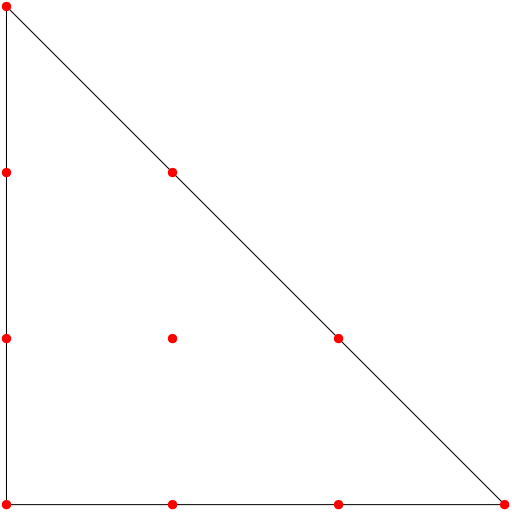
\includegraphics[scale=0.25]{resources/polynomials.png}
    \end{figure}

\end{frame}

\begin{frame}{Quantisation Dimension}

    \begin{itemize}
    \item Degree $k$ of the polynomial analogous to quantised ``energy'' of the system.
    \item Quantisation dimension $M$ equals the lattice point count (how many wavefunctions there are).
    \end{itemize}

    \begin{figure}
        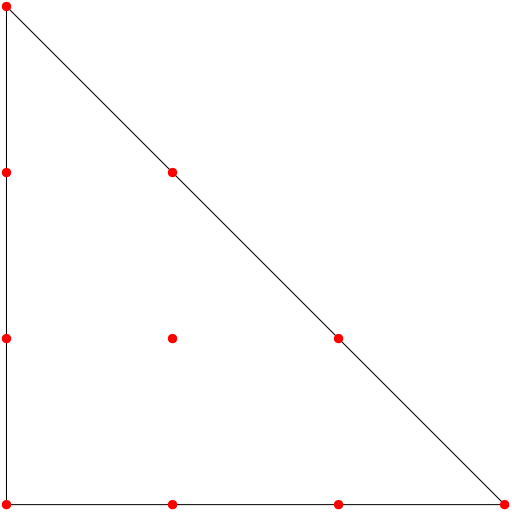
\includegraphics[scale=0.25]{resources/polynomials.png}
    \end{figure}

\end{frame}

\begin{frame}{Combinatorics}

    \begin{itemize}
       \item Useful to view the polytope as an intersection of half-spaces.
    \end{itemize}

    \begin{figure}
        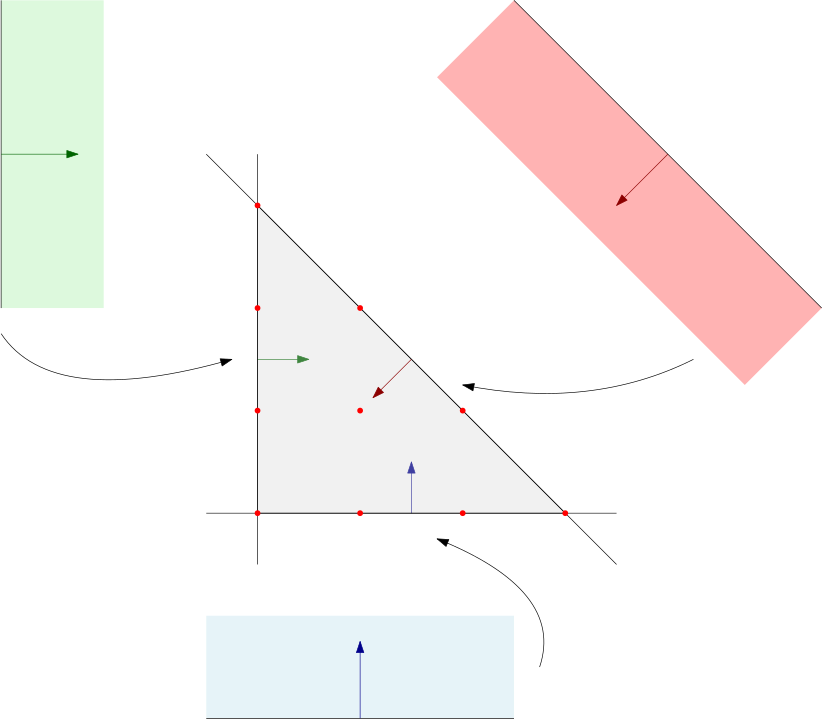
\includegraphics[scale=0.25]{resources/half-spaces.png}
    \end{figure}

\end{frame}